\documentclass[12pt,a4paper]{article}

\usepackage[a4paper,text={16.5cm,25.2cm},centering]{geometry}
\usepackage{lmodern}
\usepackage{amssymb,amsmath}
\usepackage{bm}
\usepackage{graphicx}
\usepackage{microtype}
\usepackage{hyperref}
\usepackage{minted}
\setlength{\parindent}{0pt}
\setlength{\parskip}{1.2ex}

\hypersetup
       {   pdfauthor = {  },
           pdftitle={  },
           colorlinks=TRUE,
           linkcolor=black,
           citecolor=blue,
           urlcolor=blue
       }






\begin{document}



\subsection{Spektralno razvrščanje v gruče}
Spektralno razvrščanje v gruče uporabi Laplaceovo matriko (\texttt{L}) podobnostnega grafa podatkov, da podatke preslika v prostor kjer jih je lažje razvrstiti. Algoritem deluje tako, da najprej poiščemo k najmanjših lastnih vrednosti za \texttt{L}. \texttt{Q = [v\_1,v\_2,...,v\_k]} je matrika lastnih vektorjev. Za stolpce \texttt{Q\^{}T} izvedemo algoritem k-povprečij.


\begin{minted}[texcomments = true, mathescape, fontsize=\small, xleftmargin=0.5em]{julia}
using Vaje08 # To so pravzaprav vaje06, napačno sem jih že prej generiral.
\end{minted}

Sprva generiramo oblak točk v ravnini


\begin{minted}[texcomments = true, mathescape, fontsize=\small, xleftmargin=0.5em]{julia}
using Plots
using Random
m = 100;
Random.seed!(12)
x = [1 .+ randn(m, 1); -3 .+ randn(m,1); randn(m,1)];
y = [-2 .+ randn(m, 1); -1 .+ randn(m,1); 1 .+ randn(m,1)];
scatter(x, y, title="Oblak točk v ravnini")
\end{minted}
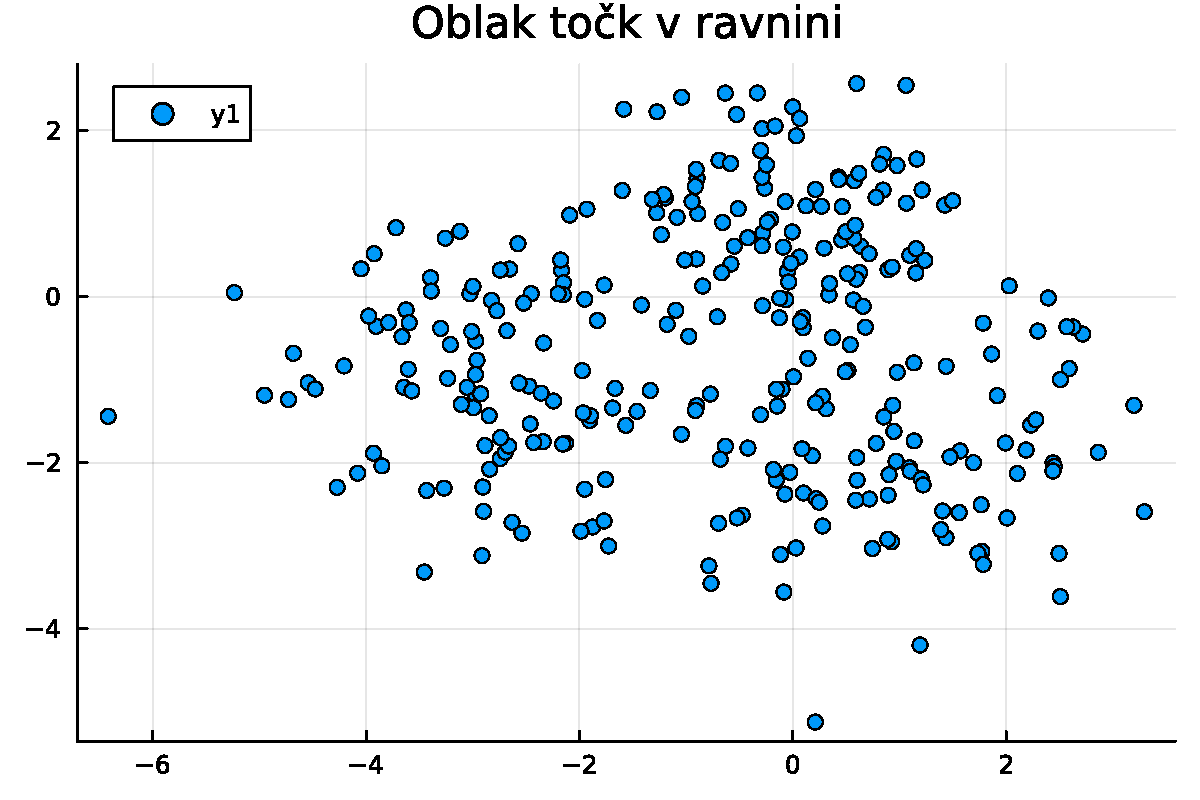
\includegraphics[width=\linewidth]{jl_Y5bBlk/demo_2_1.pdf}

Tedaj ustvarimo Laplaceovo matriko na podlagi inverzne potenčne metode, ki se uporablja zato da dobimo le nekaj najnižjih lastnih vrednosti.


\begin{minted}[texcomments = true, mathescape, fontsize=\small, xleftmargin=0.5em]{julia}
using SparseArrays
tocke = hcat(x,y)'
r = 1.4
G = graf_eps(tocke, r)
L = laplace(G)
spy(sparse(Matrix(L)), title="Porazdelitev neničelnih elementov v laplaceovi matriki")
\end{minted}
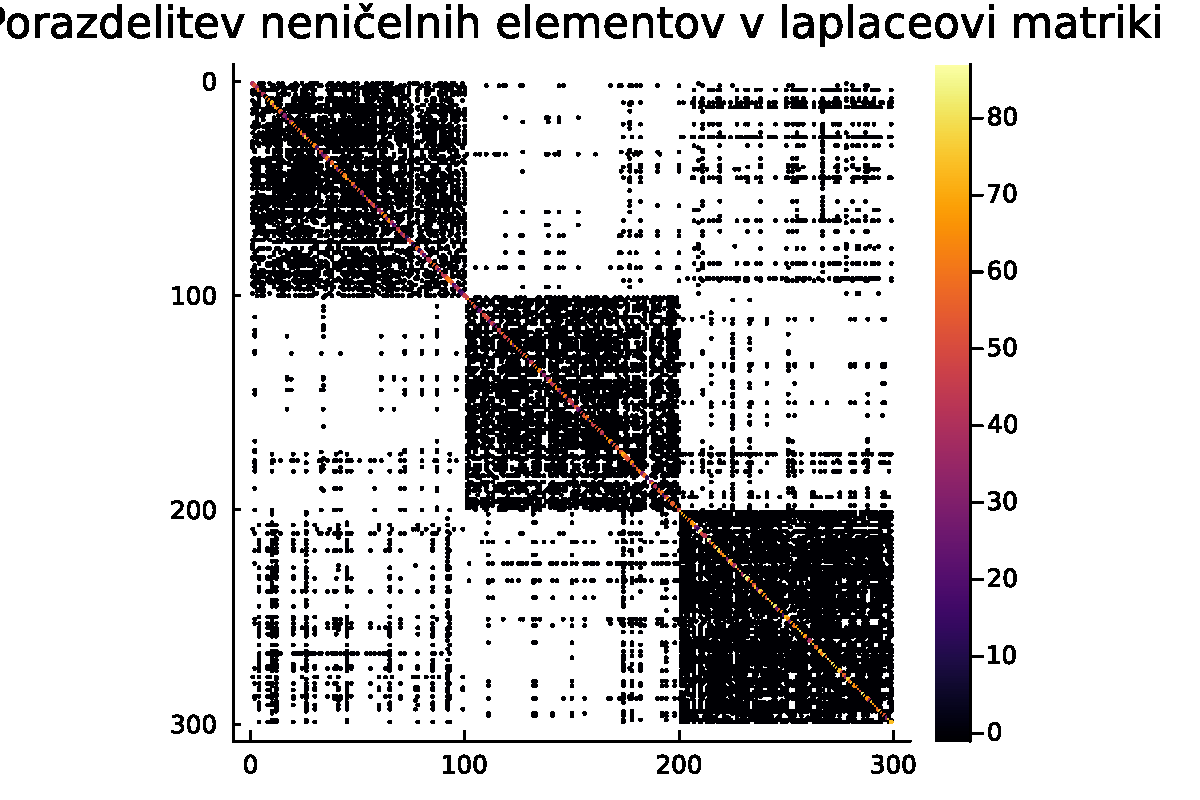
\includegraphics[width=\linewidth]{jl_Y5bBlk/demo_3_1.pdf}

Izračunamo prvih 20 lastnih vrednosti


\begin{minted}[texcomments = true, mathescape, fontsize=\small, xleftmargin=0.5em]{julia}
import LinearAlgebra.eigen
razcep = eigen(Matrix(L))
scatter(razcep.values[1:20], title="Prvih 20 lastnih vrednosti laplaceove matrike")
scatter(razcep.vectors[:,4], razcep.vectors[:,5], title="Vložitev s komponentami 4. in 5. lastnega vektorja")
\end{minted}
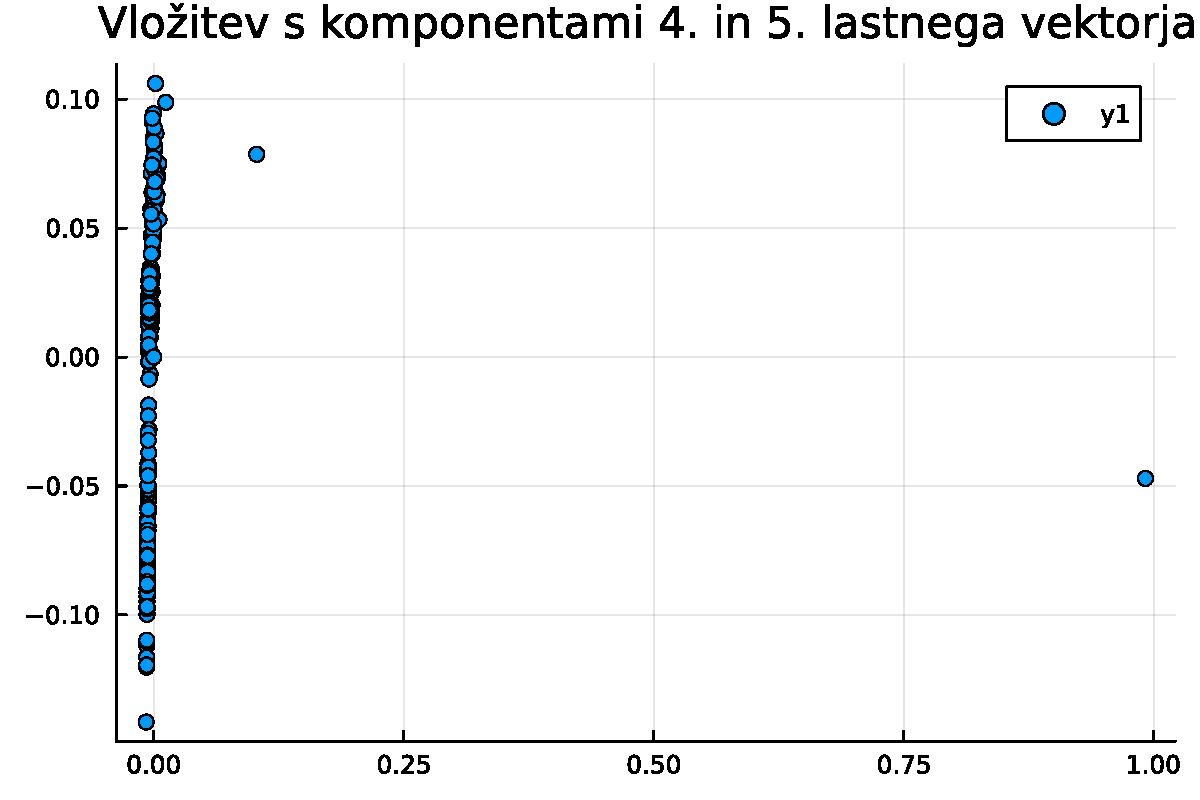
\includegraphics[width=\linewidth]{jl_Y5bBlk/demo_4_1.pdf}

Zgleda, kot da je matrika L napačno generirana saj graf vložitvje 4. in 5. lastnega vektorja ne izgleda pravilno


Sedaj pa uporabimo še clustering funkcijo kmeans, da izračunamo clusterje na podlagi podobnostnega grafa.


\begin{minted}[texcomments = true, mathescape, fontsize=\small, xleftmargin=0.5em]{julia}
using Clustering
nove_tocke = hcat(razcep.vectors[:,4],razcep.vectors[:,5])'
gruce = kmeans(nove_tocke, 3).assignments
\end{minted}
\begin{minted}[texcomments = true, mathescape, fontsize=\small, xleftmargin=0.5em, frame = leftline]{text}
300-element Vector{Int64}:
 1
 1
 1
 1
 1
 1
 2
 1
 1
 1
 |$\ensuremath{\vdots}$|
 1
 1
 1
 1
 1
 1
 1
 1
 1
\end{minted}

Originalen graf


\begin{minted}[texcomments = true, mathescape, fontsize=\small, xleftmargin=0.5em]{julia}
p1 = scatter(tocke[findall(gruce .== 1)], color=:blue, title="Originalne točke")
scatter!(p1, tocke[findall(gruce .== 2)], color=:red)
scatter!(p1, tocke[findall(gruce .== 3)], color=:green)
\end{minted}
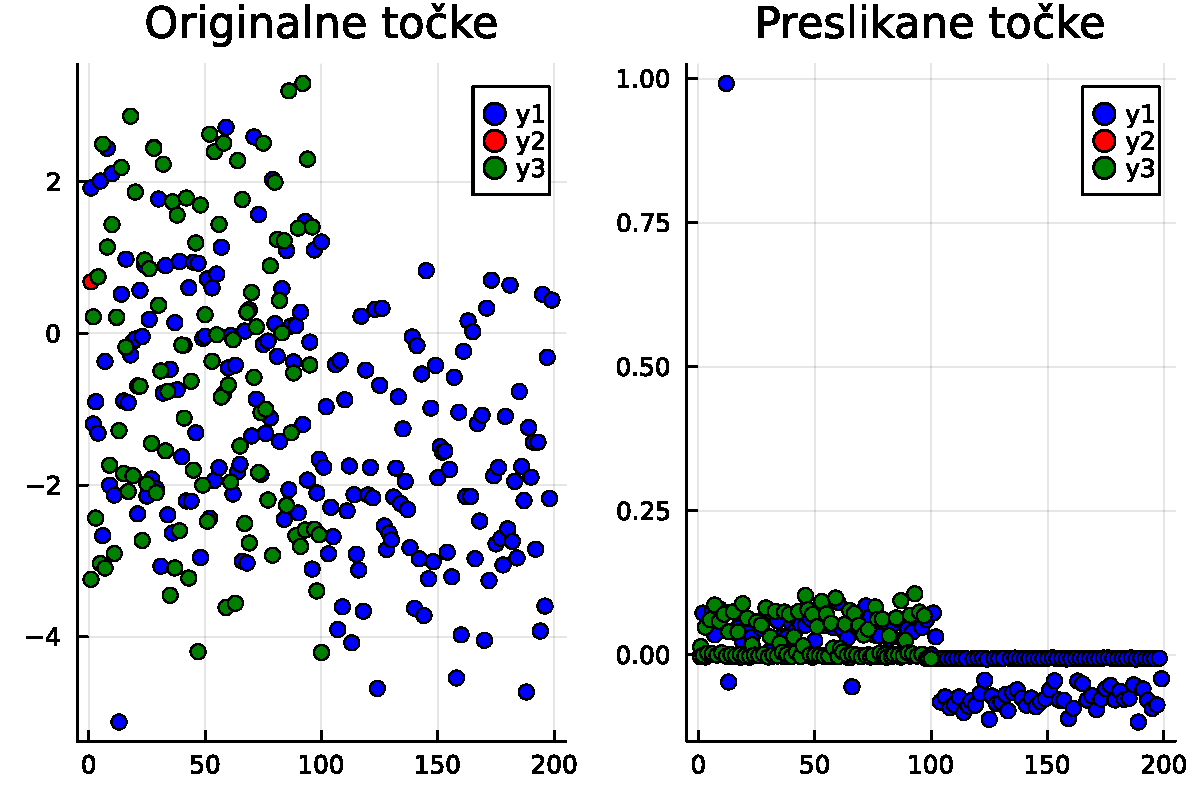
\includegraphics[width=\linewidth]{jl_Y5bBlk/demo_6_1.pdf}

Graf podobnosti


\begin{minted}[texcomments = true, mathescape, fontsize=\small, xleftmargin=0.5em]{julia}
p2 = scatter(nove_tocke[findall(gruce .== 1)], color=:blue, title="Preslikane točke")
scatter!(p2, nove_tocke[findall(gruce .== 2)], color=:red)
scatter!(p2, nove_tocke[findall(gruce .== 3)], color=:green)

plot(p1,p2)
\end{minted}
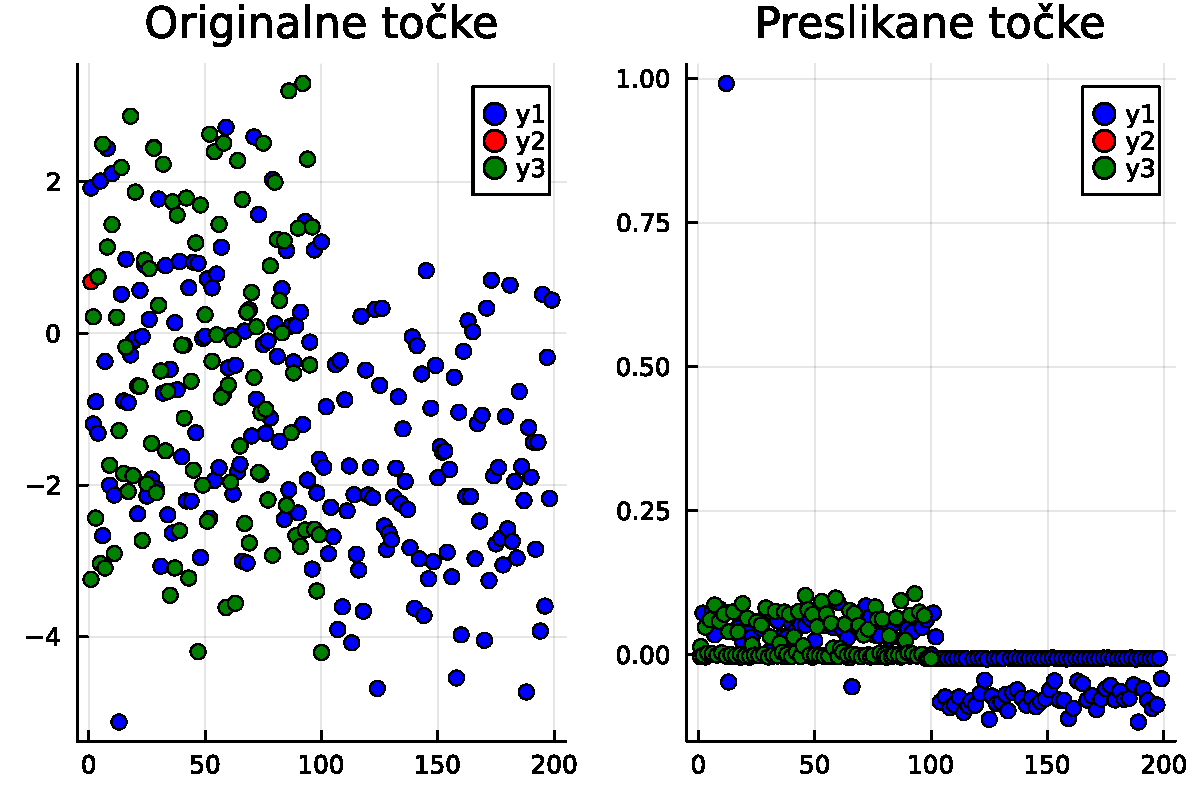
\includegraphics[width=\linewidth]{jl_Y5bBlk/demo_6_1.pdf}


\end{document}
